\section{Resilience Metrics}\label{resilience-metrics}

With increasing frequency and severity of extreme weather events (e.g., heat
waves), it is crucial to ensure urban buildings and infrastructure are resilient
to provide critical services to preserve human life and properties during
natural disasters. Building resilience has the opportunity to become an
additional value proposition for technologies and systems if it can be reliably
quantified, valued, and trusted by stakeholders. Metrics or an assessment of
potential vulnerability, likelihood, and consequence for each risk would help to
prioritize further consideration of these risk factors of building resilience
[1]. Measuring the resilience of buildings help owners make better decisions and
protect their assets, better assess the built environment resilience of larger
geographic units such as communities and cities, and complement existing
assessments of building sustainability.

The following metrics are added in EnergyPlus as optional report variables and
summary tables in three aspect: thermal, visual, and $CO_{2}$ resilience. Each
metric can be calculated and reported when users declare it as an input. The
selected resilience metrics (e.g., thermal metrics: Heat Index, Humidex, and
SET) are well defined, calculable, and have been adopted by government agency
and industry.

\subsection{Thermal Resilience}\label{thermal-resilience}

\subsubsection{Heat Index}\label{heat-index}

The heat index (HI) is an index that combines air temperature and relative
humidity (Steadman 1979), in shaded areas, to posit a human-perceived equivalent
temperature, as how hot it would feel if the humidity were some other value in
the shade. The HI measures the temperature feels like to the human body when
relative humidity is combined with the air temperature. HI is widely used in the
United States. The Occupational Safety and Health Administration (OSHA) uses HI
as an indicator to assess heat stress [2]. This has important considerations for
the human body's comfort. When the body gets too hot, it begins to perspire or
sweat to cool itself off. If the perspiration is not able to evaporate, the body
cannot regulate its temperature. When the atmospheric moisture content (i.e.
relative humidity) is high, the rate of evaporation from the body decreases. In
other words, the human body feels warmer in humid conditions. The opposite is
true when the relative humidity decreases because the rate of perspiration
increases.

Table 1 developed by U.S. National Oceanic and Atmospheric Administration (NOAA)
is used to look up the heat index by temperature (\si{\celsius}) and relative
humidity (\%) [3]. The HI effects on human health are categorized at five
levels: Safe, Caution, Extreme caution, Danger and Extreme danger, defined in
Table ~\ref{table:heat-index-chart} and color coded in Figure
~\ref{fig:heat-index-lookup-table}.

\begin{figure}[hbtp] 
\centering
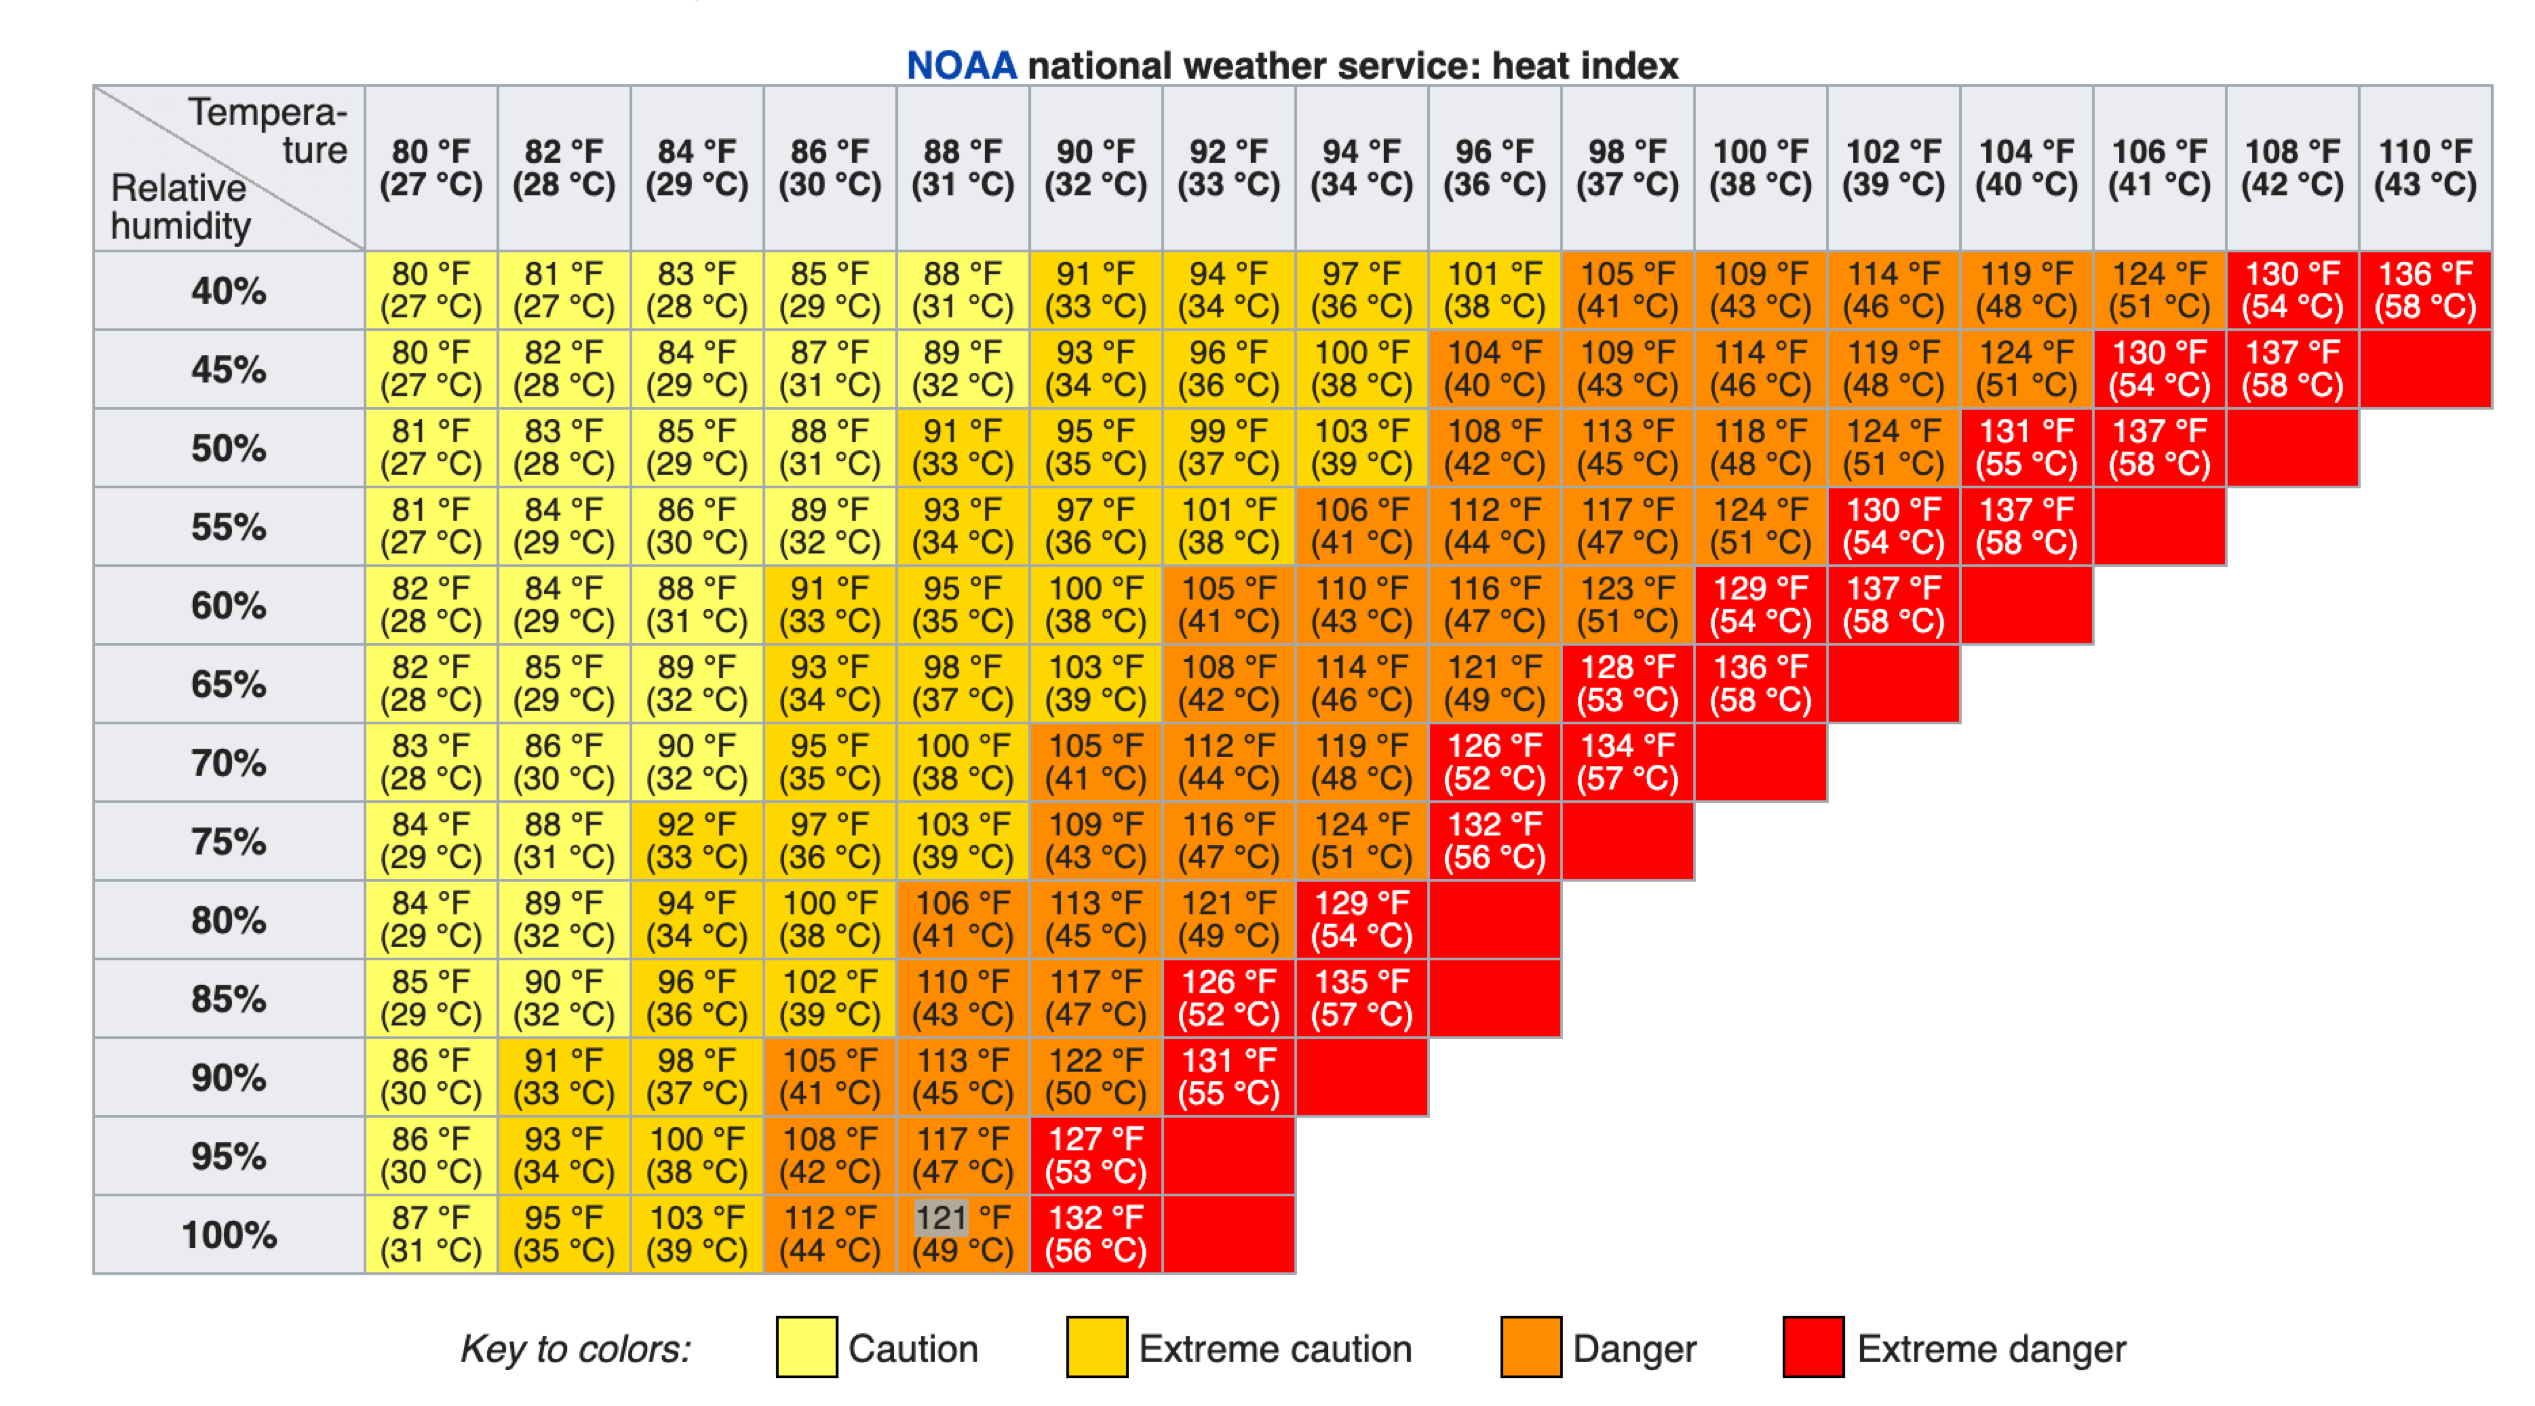
\includegraphics[width=0.9\textwidth, height=0.9\textheight, keepaspectratio=true]{media/heat_index_chart.png}
\caption{Heat Index lookup table \protect \label{fig:heat-index-lookup-table}}
\end{figure}

\begin{table}
\centering
\caption{Definition of four levels of Heat Index \label{table:heat-index-chart}} \tabularnewline
\begin{tabular}{ |p{1in}|p{1in}|p{2in}|  }
\hline
    \textbf{Heat Index in Celsius} & \textbf{Heat Index in Fahrenheit} & \textbf{Heat Index Level} \\ \hline 
    Less than \SI{26.7}{\celsius} & Less than \IP{80}{\fahrenheit} & Safe: no risk of heat hazard \\ \hline
    \SI{26.7}{\celsius} - \SI{32.2}{\celsius} & \IP{80}{\fahrenheit} - \IP{90}{\fahrenheit} & Caution: fatigue is possible with prolonged exposure and activity. Continuing activity could result in heat cramps. \\ \hline
    \SI{32.2}{\celsius} - \SI{39.4}{\celsius}& \IP{90}{\fahrenheit} – \IP{103}{\fahrenheit} & Extreme caution: heat cramps and heat exhaustion are possible. Continuing activity could result in heat stroke. \\ \hline
    \SI{39.4}{\celsius} - \SI{51.7}{\celsius} & \IP{103}{\fahrenheit} - \IP{125}{\fahrenheit} & Danger: heat cramps and heat exhaustion are likely; heat stroke is probable with continued activity. \\ \hline
    over \SI{51.7}{\celsius} & over \IP{125}{\fahrenheit} & Extreme danger: heat stroke is imminent. \\ \hline
\end{tabular}
\end{table}

The computation of the heat index is a refinement of a result obtained by
multiple regression analysis carried out by Lans P. Rothfusz and described in a
1990 National Weather Service (NWS) Technical Attachment (SR 90-23) [4-5]. The
calculation is based on degree Fahrenheit.

The regression equation of Rothfusz is
\begin{equation}  \label{eq:rm-1}
HI = c_1 + c_2T + c_3R + c_4TR + c_5T^2 + c_6R^2 + c_7T^2R + c_8TR^2 + c_9T^2R^2
\end{equation}

where

HI = heat index (expressed as an apparent temperature in degrees Fahrenheit),

T = ambient dry-bulb temperature (in degrees Fahrenheit),

R = relative humidity (percentage value between 0 and 100),

$c_1$ = -42.379,

$c_2$ = 2.04901523,

$c_3$ = 10.14333127,

$c_4$ = -0.22475541,

$c_5$ = -0.00683783,

$c_6$ = -0.05481717,

$c_7$ = 0.00122874,

$c_8$ = 0.00085282,

$c_9$ = -0.00000199.

If the RH is less than 13\% and the temperature is between 80 and \IP{112}{\fahrenheit}, then
the following adjustment is subtracted from HI:

\begin{equation}  \label{eq:rm-2}
HI = (13 - R) / 4 * ((17 - |T - 95|) / 17)^{0.5}
\end{equation}

Otherwise, if the RH is greater than 85\% and the temperature is between 80 and
\IP{87}{\fahrenheit}, then the following adjustment is added to HI:

\begin{equation}  \label{eq:rm-3}
HI = (R - 85) / 10 * (87 - T) / 5
\end{equation}

The Rothfusz regression is not appropriate when conditions of temperature and
humidity warrant a heat index value below about \IP{80}{\fahrenheit}. In those cases, a simpler
formula is applied to calculate values consistent with Steadman's results:

\begin{equation}  \label{eq:rm-4}
HI = 0.5 * (T + 61.0 + (T - 68.0) * 1.2 + (R * 0.094))
\end{equation}

In practice, the simple formula is computed first based on the temperature and
humidity. If this heat index value is \IP{80}{\fahrenheit} or higher, the full regression
equation along with any adjustment as described above is applied. The Rothfusz
regression is not valid for extreme temperature and relative humidity conditions
beyond the range of data considered by Steadman.

The Heat Index Hours (accumulated hours for a space) and Heat Index
OccupantHours (accumulated hours for the sum of all occupants in a space) of
each level for each zone and the whole building are reported under the Annual
Thermal Resilience Report.

\subsubsection{Humidex}\label{humidex}

The humidex (short for humidity index) is an index number used by Canadian
meteorologists to describe how hot the weather feels to the average person, by
combining the effect of heat and humidity. The term humidex was first coined in
1965 [6]. The humidex is a nominally dimensionless quantity (though generally
recognized by the public as equivalent to the degree Celsius) based on the
dew-point temperature [7].

The Humidex effects on human health are categorized at five levels: Little to no
discomfort, Some discomfort, Great discomfort; avoid exertion, Dangerous and
Heat stroke imminent, defined in Table ~\ref{table:humidex-chart} and color
coded in Figure ~\ref{fig:humidex-lookup-table}.

\begin{figure}[hbtp] 
\centering
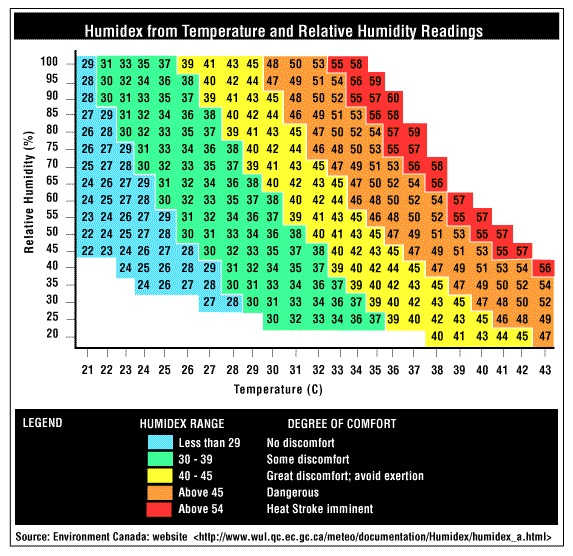
\includegraphics[width=0.9\textwidth, height=0.9\textheight, keepaspectratio=true]{media/humidex_chart.jpg}
\caption{Humidex lookup table \protect \label{fig:humidex-lookup-table}}
\end{figure}

\begin{table}
\centering
\caption{Definition of five levels of Humidex \protect \label{table:humidex-chart}} \tabularnewline
\begin{tabular}{ |p{1in}|p{3in}|  }
\hline
      \textbf{Humidex Value} & \textbf{Humidex Level} \\ \hline
      Below 29 & Little to no discomfort \\ \hline
      29 to 40 & Some discomfort \\ \hline
      40 to 45 & Great discomfort; avoid exertion \\ \hline
      45 to 50 & Dangerous \\ \hline
      Above 50 & Heat stroke imminent \\ \hline
\end{tabular}
\end{table}

The humidex (H) formula is:

\begin{equation}  \label{eq:rm-5}
H = T_{air} + \frac{5}{9}(6.11 * exp^{5417.7530 * (\frac{1}{273.16} - \frac{1}{273.15 + T_{dew}})} - 10)
\end{equation}

Where,

$H$ = the Humidex,

$T_{air}$ = the air temperature in \si{\celsius},

$T_{dew}$ = the dew-point temperature in \si{\celsius},

$exp$ = 2.71828.

The Humidex Hours (accumulated hours for a space) and Humidex OccupantHours
(accumulated hours for the sum of all occupants in a space) of each level for
each zone and the whole building are reported under the Annual Thermal
Resilience Report.

\subsubsection{Standard Effective Temperature Hours}\label{set-hour}
Standard Effective Temperature (SET) is a model of human response to the thermal
environment. Developed by A.P. Gagge and accepted by ASHRAE in 1986, SET is also
referred to as the Pierce Two-Node model [8]. Its calculation is similar to PMV
because it is a comprehensive comfort index based on heat-balance equations that
incorporate personal factors of clothing and metabolic rate. Its fundamental
difference is it takes a two-node method to represent human physiology in
measuring skin temperature and skin wettedness. ASHRAE 55-2010 defines SET as
``the temperature of an imaginary environment at 50\% relative humidity, $<$ 0.1
m/s [0.33 ft/s] average air speed, and mean radiant temperature equal to average
air temperature, in which total heat loss from the skin of an imaginary occupant
with an activity level of 1.0 met and a clothing level of 0.6 clo is the same as
that from a person in the actual environment, with actual clothing and activity
level'' [9].

LEED Pilot Credit IPpc100 - Passive Survivability and Back-up Power During
Disruptions - defines ``Livable conditions'' as SET between \IP{54}{\fahrenheit} and
\IP{86}{\fahrenheit}. The credit requires buildings to maintain safe thermal
conditions in the event of an extended power outage or loss of heating fuel, or
provide backup power to satisfy critical loads. Accumulated SET-degree-days and
SET-hours are metrics to measure thermal safety and temperatures. The SET-degree-days
and SET-degree-hours are in Celsius/Fahrenheit degrees days/hours based on the indoor SET.

LEED Passive Survivability defines the Thermal Safety Temperatures for Path 2
using the SET:

\begin{itemize}
\item Cooling: Not to exceed \IP{9}{\fahrenheit}$\cdot$day SET-degree-days (\IP{216}{\fahrenheit}$\cdot$hr SET-degree-hours)
  above \IP{86}{\fahrenheit} for residential buildings. (SI Metric: Not to exceed
  \SI{5}{\celsius}$\cdot$day SET-degree-days (\SI{120}{\celsius}$\cdot$hr SET-degree-hours) above
  \SI{30}{\celsius} SET for residential buildings.)
\item Cooling: Not to exceed \IP{18}{\fahrenheit}$\cdot$day SET-degree-days (\IP{432}{\fahrenheit}$\cdot$hr SET-degree-hours)
  above \IP{86}{\fahrenheit} SET for non-residential buildings. (SI Metric: Not to
  exceed \SI{10}{\celsius}$\cdot$day SET-degree-days (\SI{240}{\celsius}$\cdot$hr SET-degree-hours) above
  \SI{30}{\celsius} SET for non-residential buildings.)
\item Heating: Not to exceed \IP{9}{\fahrenheit}$\cdot$day SET-degree-days (\IP{216}{\fahrenheit}$\cdot$hr SET-degree-hours
  for all buildings. (SI Metric: Not to exceed \SI{5}{\celsius}$\cdot$day SET-degree-days
  (\SI{120}{\celsius}$\cdot$hr SET-degree-hours) below \SI{12}{\celsius} SET-degree-hours for all
  buildings.)
\end{itemize}

EnergyPlus calculates and reports SET as a time-step report variable when Pierce
method is chosen as the People's thermal comfort model. The aggregated
SET-Degree-Hours Occupant-Weighted Degree-Hours, and Occupied Degree-Hour (at
zone level) for both cooling and heating are reported under the Annual Thermal
Resilience Summary. The tables also include the longest continuous unmet time
duration in hours and the start time of their occurrences during the occupied
period (first occurrence if multiple time slots have the same duration).

\subsubsection{Hours of Safety}\label{hours-of-safety}

Hours of Safety is a framework developed by EPA and RMI to help understand how
long a home can maintain thresholds of comfort and safety before reaching unsafe
indoor temperature levels [10]. The concept attempts to define the duration of
time that homes can be expected to provide safe temperatures when the power goes
out based on building characteristics and energy efficiency levels (e.g.,
insulation, infiltration). This metric can be used to quantify the amount of
time people are exposed to extremely hot or cold temperatures indoors. The
information can be used to guide weatherization efforts and emergency response
measures in considering the health and safety of vulnerable populations as
extreme weather events increase in frequency.

Hours of Safety for cold or hot weather events should be defined by the longest
duration (number of hours), starting from the beginning time of the risk period
(e.g., the start time of a power outage), to not exceed temperature thresholds
defined for a specific type of population (e.g., cold stress safety temperature
for the healthy population as \IP{60}{\fahrenheit}, or \SI{16}{\celsius}). To define the
thresholds, we will use EnergyPlus's existing thermal comfort model controlled
primarily by the People input object, and add two fields in the People object,
namely ``Cold Stress Temperature Threshold'' and ``Heat Stress Temperature
Threshold''. The risk period is specified in the Output:Table:ReportPeriod object (details available in the InputOutputReference document.

The default ``Cold Stress Temperature Thresholds'': \IP{60}{\fahrenheit} (\SI{16}{\celsius})
for the healthy population [10]. Other values can be used: \IP{64}{\fahrenheit}
(\SI{18}{\celsius}) for the elderly [10], and \IP{71}{\fahrenheit} (\SI{22}{\celsius}) for nursing
home residents [11]. The default ``Hot Stress Temperature Threshold'' is
selected as \IP{86}{\fahrenheit} (\SI{30}{\celsius}) [11]. Users can modify these default
thresholds with the ``Cold Stress Temperature Threshold'' and ``Heat Stress
Temperature Threshold'' input fields in the People object.

\subsubsection{Setpoint Unmet Degree-Hours}\label{unmet-degree-hours}

The concept of UDH is analogous to that of temperature-weighted exceedance
hours, a metric defined in Section L.3.2.2(b) of ASHRAE Standard 55–2020 [12].
The UDH metric is based on indoor cooling or heating setpoint and weights each
hour that the temperature of a conditioned zone exceeds a certain threshold by
the number of degrees Celsius by which it surpasses that threshold. Compared
with average temperature or unmet hours, UDH provides a more complete picture of
the overall history of temperature exceedance.

The UDH is calculated as follows:

\begin{equation}\label{eq:udh}
\text{UDH} = \int_{t_1}^{t_2}[T(t) - T_{\text{threshold}}]_+dt
\end{equation}

where $T$ is the indoor air temperature [\si{\celsius}]; $t$ is time [h]; and $x_+ = x$
if $x > 0$, or 0 otherwise. $T_{\text{threshold}}$ is the indoor cooling or heating setpoint
[\si{\celsius}] in both the grid-on and grid-off scenarios. A similar metric, the
Exceedance Degree-Hour, is recently developed by Salimi et al [13]. Instead of
thresholding, this metric weights each hour by the distance from the current SET
to the comfort zone [13].

\subsubsection{Discomfort-weighted
Exceedance}\label{discomfort-weighted-exceedance}

Discomfort-weighted exceedance hours is the sum of the positive values of
predicted mean vote (PMV) exceedance during occupied hours, where PMV exceedance
= (PMV – threshold) for warm or very-hot conditions, and PMV exceedance =
(threshold - PMV) for cool or very-cold conditions [14]. Warm, cool, very-hot,
and very-cold exceedance hours are the number of hours in which occupants are
uncomfortably warm (PMV>0.7), cool (PMV<−0.7), very hot (PMV>3), and very cold
(PMV<−3). For example, discomfort-weighted warm exceedance hour is the sum of
the positive values of (PMV - 0.7) during occupied hours, while
discomfort-weighted cool exceedance hour is the sum of the positive values of
(-0.7 - PMV) during occupied hours. Discomfort-weighted very-hot and very-cold
exceedance hours are calculated analogously, using thresholds of 3 and -3,
respectively. CBE developed an online tool to compute thermal comfort metrics
including PMV, PPD, thermal sensation, SET, etc [15].

\subsection{Indoor Air Quality - CO2
Resilience}\label{indoor-air-quality-resilience}

For indoor air quality, we chose to use $CO_2$ concentration at the zone level
as an indicator. $CO_2$ at very high concentrations (e.g., greater than 5,000
ppm) can pose a health risk, referring to Appendix D Summary of Selected Air
Quality Guidelines in ASHRAE Standard 62.1-2016, ``Ventilation for Acceptable
Indoor Air Quality''. At concentrations above 15,000 ppm, some loss of mental
acuity has been noted. The Occupational Safety and Health Administration (OSHA)
of the US Department of Labor defined the Permissible Exposure Limits (PEL) and
Short-Term Exposure Limit (STEL) of $CO_2$ level to be 5,000 ppm and 30,000 ppm
accordingly [16].

$CO_2$ increases in buildings with higher occupant densities, and is diluted and
removed from buildings with outdoor air ventilation. High $CO_2$ levels may
indicate a problem with overcrowding or inadequate outdoor air ventilation.
Thus, maintaining a steady-state $CO_2$ concentration in a space no greater than
about 700 ppm above outdoor air levels will indicate that a substantial majority
of visitors entering a space will be satisfied with respect to human
bio-effluents (body odor). With outdoor $CO_2$ concentration varies from 350 to
500 ppm, we assume 1000 ppm is the safe threshold of indoor $CO_2$
concentration.

EnergyPlus calculates and reports the Zone Air $CO_2$ Concentration [ppm] as a
report variable, and the thresholds of different levels defined in Table
~\ref{table:co2-lvel-chart}. The Annual CO2 Resilience summary reports the Hours
and OccupantHours of each level for each zone and the whole building.

\begin{table} \centering
\caption{Indoor $CO_2$ levels required at various health conditions
\protect \label{table:co2-lvel-chart}} \tabularnewline
\begin{tabular}{ |p{2in}|p{2in}| } \hline \textbf{Indoor $CO_2$ Concentration }
& \textbf{$CO_2$ Level} \\ \hline $<=$ 1000 ppm & Normal \\ \hline $<=$ 5,000
ppm and $>$ 1000 ppm & Caution \\ \hline $>$ 5,000 ppm & Hazard \\ \hline
\end{tabular}
\end{table}

To activate the $CO_2$ concentration calculation in EnergyPlus, the
\textbf{ZoneAirContaminantBalance} object needs to be specified and with the
field \textbf{``Carbon Dioxide Concentration''} set to Yes. Users can define a
schedule of outdoor air $CO_2$ concentration in the field \textbf{``Outdoor
Carbon Dioxide Schedule Name''}. $CO_2$ generation rate at the zone level can be
specified using the \textbf{ZoneContaminantSourceAndSink:CarbonDioxide} object.

\subsection{Visual Resilience}\label{visual-resilience}

Adequate indoor lighting level is crucial for occupant safety, health and
productivity. The $10^{th}$ edition of The Lighting Handbook published by IESNA
recommends illuminance levels for various types of spaces in a building. The US
General Services Administration provides lighting levels for US Government
buildings (Table ~\ref{table:lighting-level-chart}), which can be used as a
guide for other types of buildings. The required light levels are indicated in a
range because different tasks, even in the same space, require different amounts
of light. In general, low contrast and detailed tasks require more light while
high contrast and less detailed tasks require less light.

\begin{table} \centering
\caption{GSA recommended lighting levels \label{table:lighting-level-chart}}
\tabularnewline
\begin{tabular}{ |p{2in}|p{1in}|p{1in}| } \hline \textbf{Room Type} &
\textbf{Light Level (Foot Candles)} & \textbf{Light Level (Lux)} \\ 
\hline
Bedroom - Dormitory & 20-30 FC & 200-300 lux \\ 
\hline 
Cafeteria - Eating & 20-30 FC & 200-300 lux \\ 
\hline 
Classroom - General & 30-50 FC & 300-500 lux \\
\hline 
Conference Room & 30-50 FC & 300-500 lux \\ 
\hline 
Corridor & 5-10 FC & 50-100 lux \\ 
\hline Exhibit Space & 30-50 FC & 300-500 lux \\ 
\hline 
Gymnasium - Exercise / Workout & 20-30 FC & 200-300 lux \\ 
\hline 
Gymnasium - Sports / Games & 30-50 FC & 300-500 lux \\
 \hline Kitchen / Food Prep & 30-75 FC &
300-750 lux \\
 \hline Laboratory (Classroom) & 50-75 FC & 500-750 lux \\
 \hline
Laboratory (Professional) & 75-120 FC & 750-1200 lux \\
 \hline Library - Stacks
& 20-50 FC & 200-500 lux \\
 \hline Library - Reading / Studying & 30-50 FC &
300-500 lux \\
 \hline Loading Dock & 10-30 FC & 100-300 lux \\
 \hline Lobby -
Office/General & 20-30 FC & 200-300 lux \\
 \hline Locker Room & 10-30 FC &
100-300 lux \\
 \hline Lounge / Breakroom & 10-30 FC & 100-300 lux \\
 \hline
Mechanical / Electrical Room & 20-50 FC & 200-500 lux \\
 \hline Office - Open &
30-50 FC & 300-500 lux \\
 \hline Office - Private / Closed & 30-50 FC & 300-500
lux \\
 \hline Parking - Interior & 5-10 FC & 50-100 lux \\
 \hline Restroom /
Toilet & 10-30 FC & 100-300 lux \\
 \hline Retail Sales & 20-50 FC & 200-500 lux
\\
 \hline Stairway & 5-10 FC & 50-100 lux \\
 \hline Storage Room - General &
5-20 FC & 50-200 lux \\
 \hline Workshop & 30-75 FC & 300-750 lux \\
 \hline
\end{tabular}
\end{table}

For resilience reporting purpose, we chose three thresholds: a bit dark - less
than 100 lux, dim – 100 to 300 lux, adequate – 300 to 500 lux, bright – more
than 500 lux.

\begin{itemize}
\item 100 lux – This level of light is sufficient for lifts, corridors and
stairs. Areas that are transitory for occupants and don't require any detailed
work. Warehouse areas and bulk stores will also require this minimal light
level.
\item 300 lux – Assembly areas, like village halls require at least 300 lux.
\item 500 lux – Retail spaces should have this as a minimum light level, as
should general office spaces. This level should be suitable for prolonged work
on computers, machinery and reading.
\item More than 500 lux – If you have an area where intricate work is being
carried out, then very high lux values may be needed. Where fine detailed work
is being carried out, anything up to 2,000 lux can be used – this is usually
only necessary in fairly unusual circumstances.
\end{itemize}

To activate the indoor illuminance calculation in EnergyPlus, users need to
define the \textbf{Daylighting:Controls} and the
\textbf{Daylighting:ReferencePoint} objects, even if no daylighting controls are
actually implemented in the building simulation model.

The Annual Visual Resilience summary reports the Hours and OccupantHours of each
illuminance level for each zone and the whole building.

\subsection{Timespan of Report}

Resilience metrics are more often evaluated during a certain period when a
building is at risk (e.g., during the power outage event or heatwave event), and
the period is not necessarily the same as the whole simulation period. This can
be achieved through the Output:Table:ReportPeriod input object.

\subsection{References}

{[}1{]} K. Sun, M. Specian, T. Hong, Nexus of thermal resilience and energy
efficiency in buildings: A case study of a nursing home, Build. Environ. 177
(2020) 106842. doi:10.1016/j.buildenv.2020.106842.

{[}2{]} M.E. Kiersma, Occupational Safety and Health Administration, Encycl.
Toxicol. Third Ed. (2014) 642. doi:10.1016/B978-0-12-386454-3.00344-4.

{[}3{]} G. Brooke Anderson, M.L. Bell, R.D. Peng, Methods to calculate the heat
index as an exposure metric in environmental health research, Environ. Health
Perspect. 121 (2013) 1111–1119. doi:10.1289/ehp.1206273.

{[}4{]} R.G. Steadman, The assessment of sultriness. Part I. A
temperature-humidity index based on human physiology and clothing science., J.
Appl. Meteorol. 18 (1979) 861–873.
doi:10.1175/1520-0450(1979)018<0861:TAOSPI>2.0.CO;2.

{[}5{]} L.P. Rothfusz, N.S.R. Headquarters, The heat index equation (or, more
than you ever wanted to know about heat index), Fort Worth, Texas Natl. Ocean.
Atmos. Adm. Natl. Weather Serv. Off. Meteorol. (1990) 23–90.
papers://c6bd9143-3623-4d4f-963f-62942ed32f11/Paper/p395.

{[}6{]} F.R. JM Masterton, Humidex: a method of quantifying human discomfort due
to excessive heat and humidity, Print book, Environment Canada, Atmospheric
Environment, 1979.

{[}7{]} R. Rana, B. Kusy, R. Jurdak, J. Wall, W. Hu, Feasibility analysis of
using humidex as an indoor thermal comfort predictor, Energy Build. 64 (2013)
17–25. doi:10.1016/j.enbuild.2013.04.019.

{[}8{]} L.G. Gagge, A. P., Fobelets, A. P. and Berglund, A standard predictive
Index of human reponse to thermal enviroment, Am. Soc. Heating, Refrig.
Air-Conditioning Eng. (1986) 709–731.

{[}9{]} ASHRAE, ASHRAE STANDARD 55-2010: Thermal Environmental Conditions for
Human Occupancy, 2013.

{[}10{]} S. Ayyagari, M. Gartman, and J. Corvidae, ``A Framework for Considering
Resilience in Building Envelope Design and Construction,'' Feb. 2020.

{[}11{]} USGBC, ``Passive Survivability and Back-up Power During Disruptions |
U.S. Green Building Council,'' Oct. 2018.
https://www.usgbc.org/credits/passivesurvivability (accessed Oct. 26, 2021).

{[}12{]} ASHRAE, ``Thermal Environmental Conditions for Human Occupancy,'' p. 9,
Apr. 2021.

{[}13{]} S. Salimi, E. Estrella Guillén, and H. Samuelson, ``Exceedance
Degree-Hours: A new method for assessing long-term thermal conditions,'' Indoor
Air, vol. 31, no. 6, pp. 2296–2311, 2021, doi: 10.1111/ina.12855.

{[}14{]} R. Levinson et al., ``Key performance indicators for cool envelope
materials, windows and shading, natural ventilation, and personal comfort
systems,'' Nov. 10, 2020.

{[}15{]} F. Tartarini, S. Schiavon, T. Cheung, and T. Hoyt, ``CBE Thermal
Comfort Tool: Online tool for thermal comfort calculations and visualizations,''
SoftwareX, vol. 12, p. 100563, Jul. 2020, doi: 10.1016/j.softx.2020.100563.

{[}16{]} ACGIH, Threshold Limit Values (TLVs) and Biological Exposure Indices
(BEIs), 2012. doi:10.1073/pnas.0703993104.
